\chapter{REVISÃO BIBLIOGRÁFICA}\label{cap_revisao}

Este capítulo apresenta os fundamentos teóricos que sustentam o desenvolvimento do sistema proposto. Inicialmente, contextualiza-se a evolução histórica dos VANTs e suas classificações. Em seguida, descreve-se o princípio de funcionamento do quadricóptero e sua modelagem matemática. Abordam-se a representação em espaço de estados e o controle por Regulador Linear Quadrático Gaussiano (LQG). Por fim, discutem-se os algoritmos de otimização de rotas e a arquitetura de \textit{hardware} embarcado empregada.

% ================================================================
\section{VEÍCULOS AÉREOS NÃO TRIPULADOS: HISTÓRICO E CLASSIFICAÇÃO}
% ================================================================

Os Veículos Aéreos Não Tripulados (VANTs), conhecidos popularmente como \textit{drones}, tiveram seus primeiros registros em meados do século XIX. Em 1849, o exército austríaco utilizou balões não tripulados carregando explosivos para bombardear a cidade de Veneza, marcando uma das primeiras aplicações militares de aeronaves sem piloto na história \cite{mori2020, zaloga2008}. Esses veículos evoluíram continuamente ao longo dos conflitos globais; na Primeira Guerra Mundial, destaca-se o torpedo aéreo Hewitt-Sperry, guiado por giroscópio, que demonstrou a viabilidade do voo autônomo controlado por instrumentos \cite{newcome2004}. Em 1935, a Marinha Real britânica desenvolveu o \textit{DH.82B Queen Bee}, um avião rádio-controlado para treinamento de artilharia antiaérea, cuja denominação inspirou o termo \textit{drone} --- ``zangão'' em inglês --- como uma alusão à sua ``abelha-rainha'' \cite{zaloga2008, newcome2004}.

A partir da década de 1960, VANTs passaram a ser empregados sistematicamente em missões de reconhecimento e vigilância, e nas décadas seguintes consolidaram-se como ferramentas estratégicas em operações militares de larga escala \cite{ayamga2021}. A transição para aplicações civis acelerou-se na década de 2010 com o surgimento de plataformas multirrotoras comerciais acessíveis, que democratizaram o acesso à tecnologia e impulsionaram o crescimento do mercado global de VANTs \cite{sivakumar2021, kapustina2021}.

\begin{figure}[H]
    \centering
    \caption{Comparativo visual de VANTs: (a) Asa Fixa, (b) Multicóptero e (c) VTOL Híbrido.}
    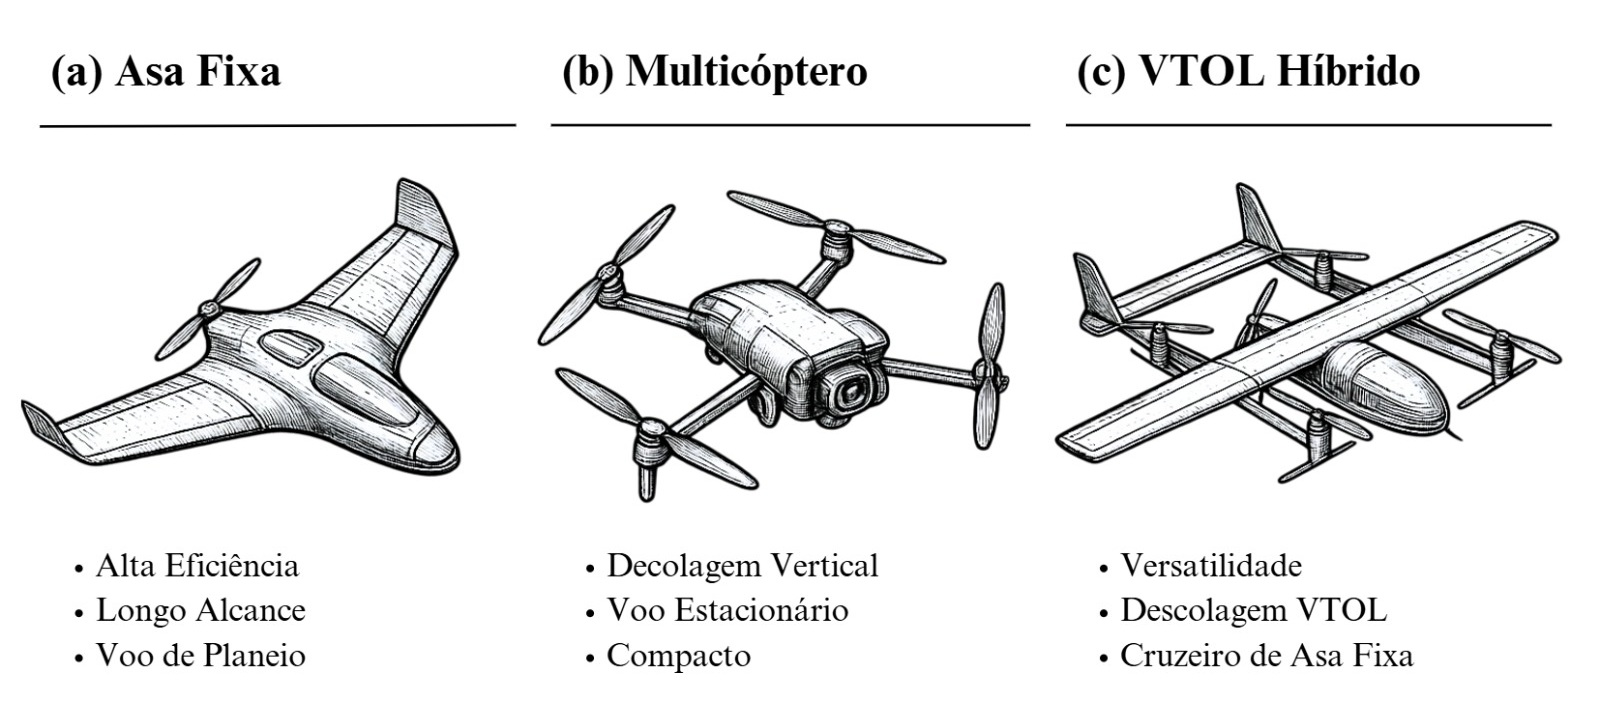
\includegraphics[width=0.8\textwidth]{images/introducao/AsaFixaMulticopteroVTOLHibrido.jpg}
    \label{fig:AsaFixaMulticopteroVTOLHibrido}
    \par\vspace{0.2cm}
    \centering\footnotesize Fonte: elaborado pelos autores (2026).
\end{figure}

Os VANTs são classificados principalmente pela sua configuração aerodinâmica, conforme ilustrado na Figura \ref{fig:AsaFixaMulticopteroVTOLHibrido}. Os modelos de Asa Fixa (a) destacam-se pela alta eficiência energética e longo alcance, sendo ideais para voos de planeio e missões de mapeamento extenso. Em contrapartida, os Multicópteros (b) oferecem a capacidade de voo estacionário e decolagem vertical em espaços compactos, embora possuam menor autonomia comparativa \cite{mohsan2023}. Por fim, os \textit{Vertical Take-Off and Landing} Híbridos (VTOLs) (c) combinam a versatilidade da decolagem vertical com a eficiência do voo de cruzeiro de asa fixa \cite{guebsi2024}.

A evolução desses veículos permitiu sua adoção em setores estratégicos. Na agricultura de precisão, VANTs possibilitam o monitoramento em tempo real de lavouras e aplicação localizada de insumos \cite{barbosajunior2024}. No setor da saúde, a tecnologia é empregada para mitigar gargalos logísticos na entrega de suprimentos vitais, como hemoderivados e medicamentos essenciais, em regiões de infraestrutura comprometida ou zonas de conflito \cite{ahmad2026}. Já na logística empresarial, o foco reside na etapa de \textit{last-mile delivery} (entrega de última milha), em que as rotas, a energia disponível e as restrições operacionais influenciam custo e nível de serviço \cite{rinaldi2024,otto2018}.

No Brasil, a Agência Nacional de Aviação Civil (ANAC) estabelece requisitos gerais para aeronaves não tripuladas de uso civil por meio do RBAC nº 100 \cite{anac2026}. O Departamento de Controle do Espaço Aéreo (DECEA), por sua vez, define procedimentos de acesso ao espaço aéreo brasileiro para sistemas de aeronaves remotamente pilotadas, incluindo critérios de solicitação, coordenação e autorização de voo \cite{decea2026}. Conceitos como \textit{Unmanned Traffic Management} (UTM) e \textit{Urban Air Mobility} (UAM) aparecem nesse contexto como temas relacionados à coordenação de operações não tripuladas e mobilidade aérea urbana, mas não substituem os requisitos normativos aplicáveis ao tipo de operação efetivamente realizado.

% ================================================================
\section{PRINCÍPIO DE FUNCIONAMENTO DE UM QUADRICÓPTERO}
% ================================================================

O quadricóptero integra a categoria de multicópteros de asas rotativas. Esse tipo de VANT possui quatro propulsores que, ao operarem em sincronia, geram o empuxo resultante necessário para realizar os movimentos de subida e descida. Adicionalmente, ao controlar a velocidade angular de cada motor individualmente, torna-se possível realizar as demais movimentações de atitude e translação. A disposição dos motores e hélices é comumente dividida nas configurações ``X'' (\textit{cross}) e ``+'' (\textit{plus}), conforme ilustrado na Figura~\ref{fig:quadrotor_flight_configurations} \cite{idrissi2022}.

\begin{figure}[H]
    \centering
    \caption{Configurações de voo de quadricópteros: (a) Plus e (b) Cross.}
    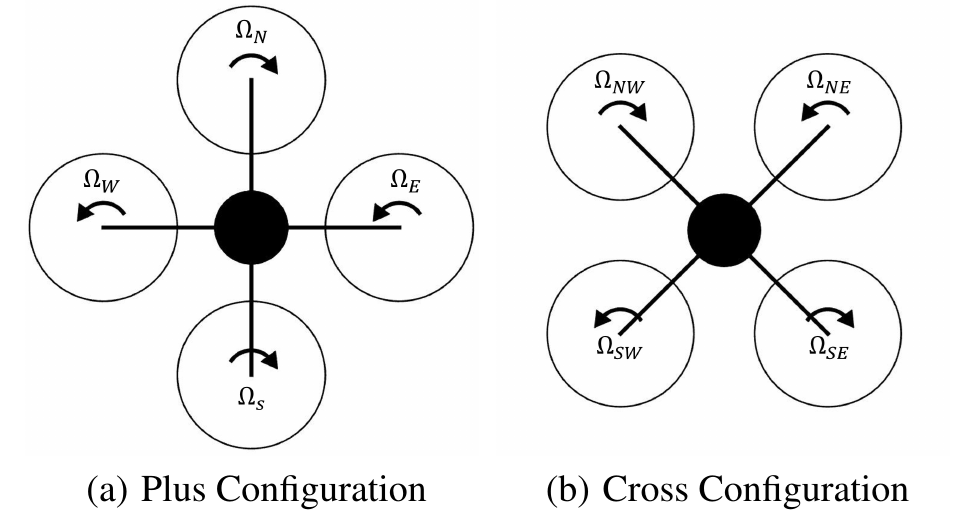
\includegraphics[width=0.8\textwidth]{images/referencial_teorico/quadrotor_flight_configurations.png}
    \label{fig:quadrotor_flight_configurations}
    \par\vspace{0.2cm}
    \centering\footnotesize Fonte: \citeonline{niemiec2016}.
\end{figure}

Em ambas as configurações, rotores adjacentes giram em sentidos opostos --- um par no sentido horário (\textit{clockwise} --- CW) e outro no sentido anti-horário (\textit{counter-clockwise} --- CCW). Essa disposição é fundamental para cancelar o torque reativo resultante da rotação das hélices, permitindo o controle do ângulo de guinada (\textit{yaw}) do veículo \cite{quan2017}. De acordo com \citeonline{niemiec2016}, nas condições analisadas pelos autores, a configuração ``X'' apresentou autoridade de controle em arfagem (\textit{pitch}) e rolamento (\textit{roll}) até aproximadamente 30\% maior que a configuração ``+''. Por essa razão, a configuração ``X'' é recorrente em plataformas comerciais e acadêmicas, sendo também a empregada neste projeto.

A movimentação do quadricóptero é governada por quatro modos de controle distintos, denominados coletivo, arfagem, rolamento e guinada, conforme descrito a seguir \cite{beard2012}:

\begin{alineastcc}
    \item \textbf{controle coletivo} ($\Omega_0$): todos os quatro motores aumentam ou diminuem a velocidade angular simultaneamente. Próximo ao voo nivelado e em uma plataforma simétrica, esse modo altera principalmente o empuxo total ($T$), com efeito direto sobre a aceleração vertical (Figura~\ref{fig:collective_control});
    \item \textbf{controle de arfagem} ($\Omega_P$): os rotores dianteiros aceleram enquanto os traseiros desaceleram (ou vice-versa), produzindo um momento em torno do eixo lateral ($y$) que inclina o veículo para frente ou para trás. Essa inclinação redireciona parte do vetor de empuxo para a horizontal, gerando aceleração longitudinal (Figura~\ref{fig:pitch_control});
    \item \textbf{controle de rolamento} ($\Omega_R$): de forma análoga ao controle de arfagem, os rotores do lado esquerdo aceleram enquanto os do lado direito desaceleram (ou vice-versa), produzindo um momento em torno do eixo longitudinal ($x$) que resulta em deslocamento lateral (Figura~\ref{fig:roll_control});
    \item \textbf{controle de guinada} ($\Omega_Y$): os rotores que giram no sentido horário (CW) aceleram enquanto os que giram no sentido anti-horário (CCW) desaceleram (ou vice-versa). Esse diferencial de torque reativo produz um momento em torno do eixo vertical ($z$), alterando a orientação do veículo (Figura~\ref{fig:yaw_control}).
\end{alineastcc}

\begin{figure}[H]
    \centering
    \caption{Controle coletivo ($\Omega_0$): variação uniforme da velocidade em todos os motores para controle de altitude.}
    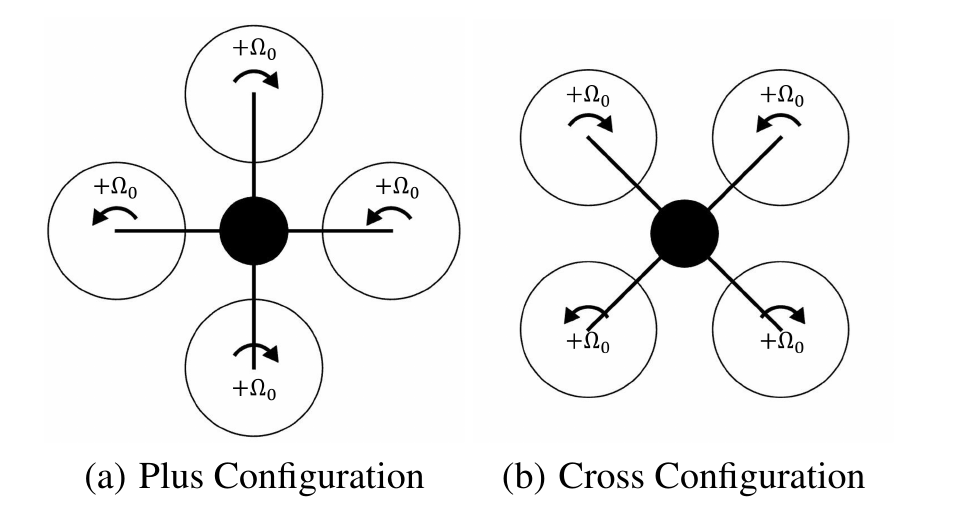
\includegraphics[width=0.8\textwidth]{images/referencial_teorico/collective_control.png}
    \label{fig:collective_control}
    \par\vspace{0.2cm}
    \centering\footnotesize Fonte: \citeonline{niemiec2016}.
\end{figure}

\begin{figure}[H]
    \centering
    \caption{Controle de arfagem ($\Omega_P$): diferencial de velocidade entre rotores dianteiros e traseiros para inclinação longitudinal.}
    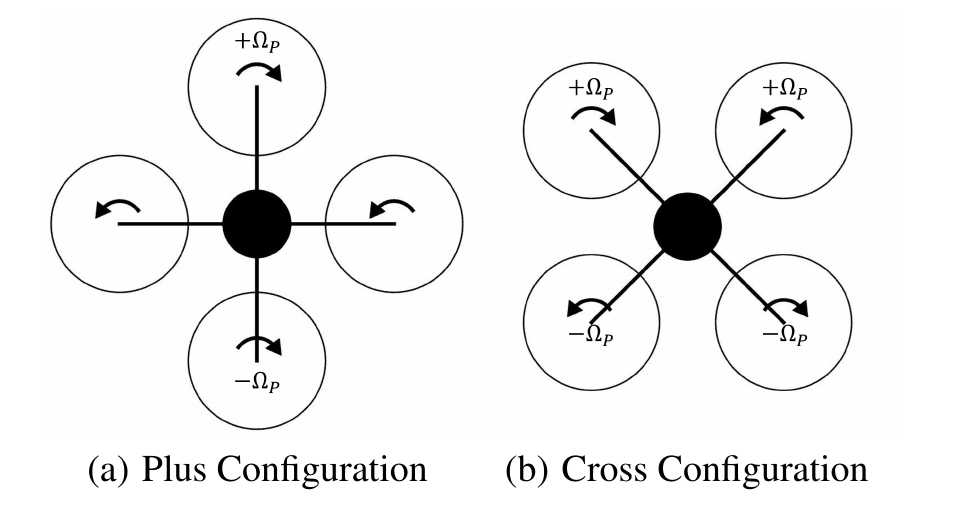
\includegraphics[width=0.8\textwidth]{images/referencial_teorico/pitch_control.png}
    \label{fig:pitch_control}
    \par\vspace{0.2cm}
    \centering\footnotesize Fonte: \citeonline{niemiec2016}.
\end{figure}

\begin{figure}[H]
    \centering
    \caption{Controle de rolamento ($\Omega_R$): diferencial de velocidade entre rotores esquerdo e direito para inclinação lateral.}
    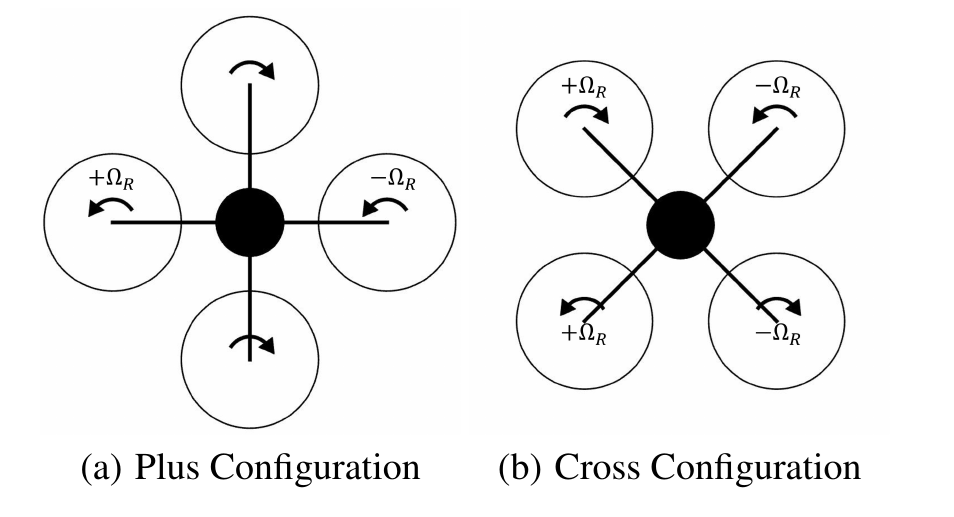
\includegraphics[width=0.8\textwidth]{images/referencial_teorico/roll_control.png}
    \label{fig:roll_control}
    \par\vspace{0.2cm}
    \centering\footnotesize Fonte: \citeonline{niemiec2016}.
\end{figure}

\begin{figure}[H]
    \centering
    \caption{Controle de guinada ($\Omega_Y$): diferencial de torque reativo entre rotores CW e CCW para rotação em torno do eixo vertical.}
    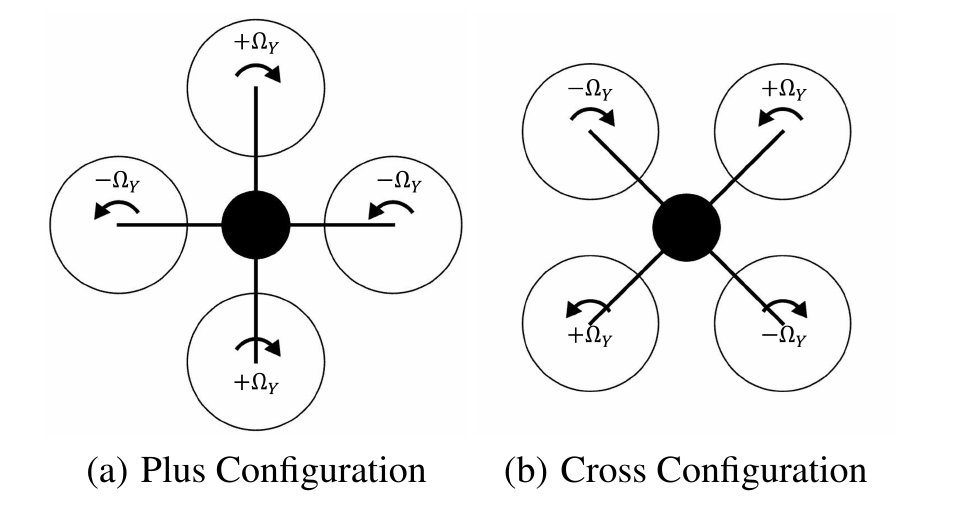
\includegraphics[width=0.8\textwidth]{images/referencial_teorico/yaw_control.png}
    \label{fig:yaw_control}
    \par\vspace{0.2cm}
    \centering\footnotesize Fonte: \citeonline{niemiec2016}.
\end{figure}

Essa decomposição dos movimentos é uma idealização útil próxima ao equilíbrio, sob hipóteses de simetria e pequenas inclinações. Conforme observado por \citeonline{idrissi2022}, essa estrutura evidencia que o quadricóptero é um sistema \textit{subatuado}: com apenas quatro entradas de controle, buscam-se controlar seis graus de liberdade --- três de translação ($x$, $y$, $z$) e três de rotação ($\phi$, $\theta$, $\psi$). Essa característica impõe restrições ao controle simultâneo de todas as variáveis e motiva a formulação em espaço de estados empregada pelo LQR, discutida na Seção~\ref{sec:controle}.

% ================================================================
\section{MODELAGEM MATEMÁTICA DO QUADRICÓPTERO}\label{sec:modelagem}
% ================================================================

A modelagem matemática de um quadricóptero consiste em descrever formalmente as relações entre as forças geradas pelos motores e o movimento resultante do veículo. Essa etapa é fundamental para o projeto de controladores, pois fornece as equações diferenciais que governam a planta a ser controlada. Nesta seção, seguem-se as formulações apresentadas por \citeonline{quan2017} e \citeonline{beard2012}, amplamente adotadas na literatura de VANTs multirrotores.

% ----------------------------------------------------------------
\subsection{Referenciais e ângulos de Euler}\label{subsec:referenciais}
% ----------------------------------------------------------------

Para descrever o movimento de um corpo rígido no espaço tridimensional, faz-se necessário definir dois sistemas de coordenadas: o referencial inercial (fixo ao solo) e o referencial do corpo (fixo ao veículo). O referencial inercial, denotado por $\mathcal{W} = \{x_W, y_W, z_W\}$, adota a convenção NED (\textit{North-East-Down}), na qual $x_W$ aponta para o norte, $y_W$ aponta para o leste e $z_W$ aponta para baixo. O referencial do corpo, denotado por $\mathcal{B} = \{x_B, y_B, z_B\}$, adota a convenção frente--direita--baixo: $x_B$ aponta para a frente do veículo, $y_B$ para a direita e $z_B$ para baixo \cite{beard2012}.

\begin{figure}[H]
    \centering
    \caption{Representação dos referenciais inercial ($\mathcal{W}$) e do corpo ($\mathcal{B}$).}
    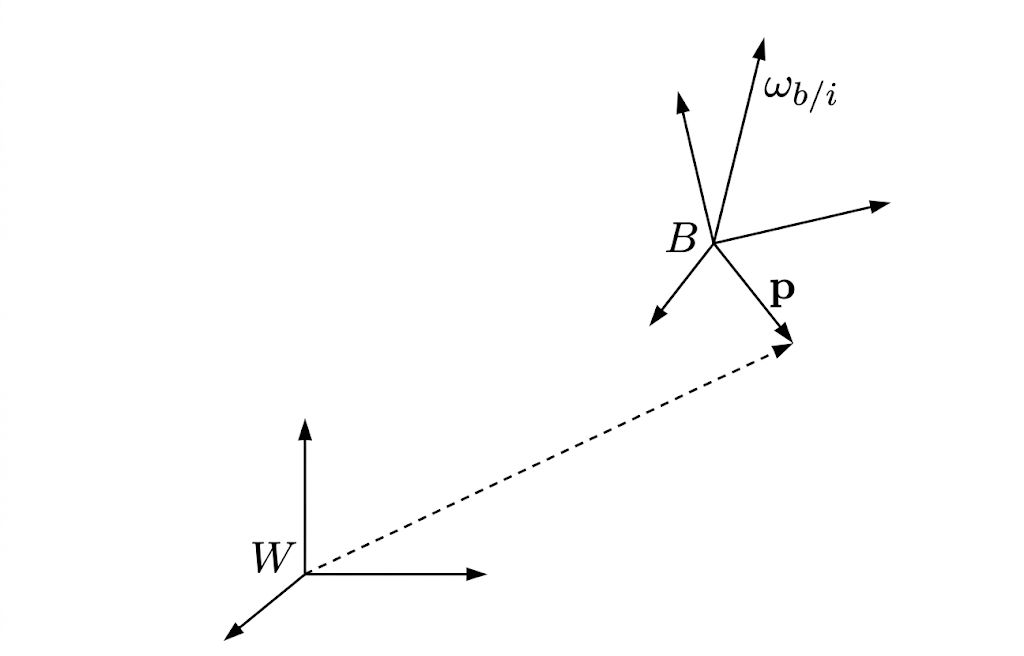
\includegraphics[width=0.6\textwidth]{images/referencial_teorico/Ref_Inercial_Corpo.jpg}
    \label{fig:referenciais_euler}
    \par\vspace{0.2cm}
    \centering\footnotesize Fonte: adaptado de \citeonline{beard2012}.
\end{figure}

A Figura~\ref{fig:referenciais_euler} representa genericamente o referencial inercial $\mathcal{W}$, o referencial do corpo $\mathcal{B}$, o vetor de posição entre eles e a velocidade angular do corpo em relação ao referencial inercial. O símbolo vetorial $\mathbf{p}$ indicado na imagem representa posição; ele não deve ser confundido com a variável escalar $p$ usada no modelo para a velocidade angular de rolamento. As direções específicas da convenção NED e dos eixos frente--direita--baixo são definidas no texto, pois a figura não identifica nominalmente cada eixo.

A orientação do referencial do corpo em relação ao referencial inercial é descrita pelos três ângulos de Euler: rolamento ($\phi$), arfagem ($\theta$) e guinada ($\psi$). A transformação entre os dois referenciais é realizada pela matriz de rotação $\mathbf{R}$, obtida pela composição de três rotações elementares na sequência ZYX \cite{quan2017}:

\begin{equation}\label{eq:rotacao}
\mathbf{R} = \mathbf{R}_z(\psi)\,\mathbf{R}_y(\theta)\,\mathbf{R}_x(\phi)
\end{equation}

\noindent resultando em:

\begin{equation}\label{eq:matriz_rotacao}
\mathbf{R} = \begin{bmatrix}
c\psi\, c\theta & c\psi\, s\theta\, s\phi - s\psi\, c\phi & c\psi\, s\theta\, c\phi + s\psi\, s\phi \\
s\psi\, c\theta & s\psi\, s\theta\, s\phi + c\psi\, c\phi & s\psi\, s\theta\, c\phi - c\psi\, s\phi \\
-s\theta & c\theta\, s\phi & c\theta\, c\phi
\end{bmatrix}
\end{equation}

\noindent onde $c(\cdot)$ e $s(\cdot)$ representam, respectivamente, cosseno e seno.

A relação entre as velocidades angulares medidas no referencial do corpo ($p$, $q$, $r$) e as taxas de variação dos ângulos de Euler ($\dot{\phi}$, $\dot{\theta}$, $\dot{\psi}$) é dada pela relação cinemática \cite{beard2012}:

\begin{equation}\label{eq:euler_rates}
\begin{bmatrix} \dot{\phi} \\ \dot{\theta} \\ \dot{\psi} \end{bmatrix} = \begin{bmatrix}
1 & s\phi\, t\theta & c\phi\, t\theta \\
0 & c\phi & -s\phi \\
0 & s\phi / c\theta & c\phi / c\theta
\end{bmatrix}
\begin{bmatrix} p \\ q \\ r \end{bmatrix}
\end{equation}

\noindent onde $t(\cdot)$ representa a tangente. Essa relação apresenta uma singularidade em $\theta = \pm 90^\circ$, conhecida como \textit{gimbal lock}. O envelope operacional adotado para o projeto deve permanecer afastado dessa singularidade; valores como $|\theta| < 15^\circ$ representam uma escolha de projeto a ser sustentada pela análise da planta não linear, e não um limite universal de validade do LQR \cite{quan2017}.

% ----------------------------------------------------------------
\subsection{Cinemática do quadricóptero}\label{subsec:cinematica}
% ----------------------------------------------------------------

A cinemática descreve a geometria do movimento sem considerar as forças que o causam. O estado completo do quadricóptero é definido por 12 variáveis agrupadas no vetor de estado \cite{beard2012}:

\begin{equation}\label{eq:vetor_estado}
\mathbf{x} = \left[ \begin{array}{cccccccccccc} 
x & y & z & \phi & \theta & \psi & \dot{x} & \dot{y} & \dot{z} & p & q & r 
\end{array} \right]^T
\end{equation}

\noindent onde $(x, y, z)$ é a posição no referencial inercial, $(\phi, \theta, \psi)$ são os ângulos de Euler, $(\dot{x}, \dot{y}, \dot{z})$ são as velocidades lineares no referencial inercial, e $(p, q, r)$ são as velocidades angulares no referencial do corpo.

As equações cinemáticas translacionais são triviais:
\begin{equation}\label{eq:cine_trans}
\dot{x} = v_x, \quad \dot{y} = v_y, \quad \dot{z} = v_z
\end{equation}

\noindent enquanto as equações cinemáticas rotacionais são dadas pela Equação~\eqref{eq:euler_rates}. Juntas, essas seis equações cinemáticas formam a primeira metade do modelo de 12 estados.

% ----------------------------------------------------------------
\subsection{Dinâmica do quadricóptero}\label{subsec:dinamica}
% ----------------------------------------------------------------

A dinâmica do quadricóptero é governada pelas leis de Newton para translação e pelas equações de Euler para rotação. Cada motor $i$ gera uma força de empuxo ($F_i$) e um torque de reação aerodinâmica ($\tau_{M,i}$) proporcionais ao quadrado de sua velocidade angular ($\omega_i$) \cite{quan2017}:

\begin{equation}\label{eq:empuxo_torque_motor}
F_i = K_t \, \omega_i^2 \quad \text{e} \quad \tau_{M,i} = K_q \, \omega_i^2
\end{equation}

\noindent onde $K_t$ é o coeficiente de empuxo (em $\mathrm{N\cdot s^2/rad^2}$) e $K_q$ é o coeficiente de torque (em $\mathrm{N\cdot m\cdot s^2/rad^2}$). O empuxo estático total ($T$) do veículo é dado pela soma dos empuxos individuais:

\begin{equation}\label{eq:empuxo_total}
T = \sum_{i=1}^{4} F_i = K_t \sum_{i=1}^{4} \omega_i^2
\end{equation}

Os torques atuantes nos três eixos do corpo são expressos em função dos esforços individuais e da geometria do veículo. Para a configuração em ``X'', define-se $d$ como a distância projetada do eixo do motor aos eixos principais de rotação (rolamento e arfagem). Em um chassi simétrico, sendo $l$ a distância radial do centro de massa até o motor, tem-se $d = l/\sqrt{2}$. 

A relação entre os esforços individuais e os esforços totais (empuxo $T$ e torques de rolamento $\tau_\phi$, arfagem $\tau_\theta$ e guinada $\tau_\psi$) é descrita por uma matriz de alocação de controle \cite{quan2017}. Definindo a constante $c = K_q$, a matriz (conhecida na literatura como \textit{motor mixing matrix}) assume a seguinte forma:

\begin{equation}\label{eq:mixing}
\begin{bmatrix} T \\ \tau_\phi \\ \tau_\theta \\ \tau_\psi \end{bmatrix}
= \begin{bmatrix}
1 & 1 & 1 & 1 \\
d & -d & -d & d \\
d & d & -d & -d \\
c & -c & c & -c
\end{bmatrix}
\begin{bmatrix} F_1 \\ F_2 \\ F_3 \\ F_4 \end{bmatrix}
\end{equation}

\noindent A correta aplicação desta matriz de mistura exige a definição prévia da disposição física dos motores, dos respectivos sentidos de rotação (horário ou anti-horário), da associação com os canais dos ESCs (\textit{Electronic Speed Controllers}) e da convenção de sinais dos momentos. De forma generalizada, para um motor localizado na coordenada $(x_i,y_i,0)$ do referencial do corpo e gerando empuxo vertical, as contribuições espaciais de torque são $\tau_{\phi,i} = y_i F_i$ e $\tau_{\theta,i} = -x_i F_i$. Por fim, a implementação prática desta alocação via protocolo DShot requer a caracterização experimental para mapear a relação não linear entre o comando digital, a tensão de alimentação e os esforços efetivamente gerados pelo conjunto motor-hélice.

Aplicando-se a Segunda Lei de Newton no referencial inercial NED, com empuxo no sentido $-z_B$ e $\mathbf{R}$ como transformação do corpo para o referencial inercial, obtém-se $m\ddot{\mathbf{r}}=mg\mathbf{e}_3-T\mathbf{R}\mathbf{e}_3$. Portanto, as equações dinâmicas translacionais são \cite{beard2012}:

\begin{equation}\label{eq:din_x}
m\ddot{x} = -T\,(c\psi\, s\theta\, c\phi + s\psi\, s\phi)
\end{equation}
\begin{equation}\label{eq:din_y}
m\ddot{y} = -T\,(s\psi\, s\theta\, c\phi - c\psi\, s\phi)
\end{equation}
\begin{equation}\label{eq:din_z}
m\ddot{z} = mg - T\, c\theta\, c\phi
\end{equation}

\noindent e as equações dinâmicas rotacionais:

\begin{equation}\label{eq:din_p}
I_{xx}\,\dot{p} = \tau_\phi - (I_{zz} - I_{yy})\,q\,r
\end{equation}
\begin{equation}\label{eq:din_q}
I_{yy}\,\dot{q} = \tau_\theta - (I_{xx} - I_{zz})\,p\,r
\end{equation}
\begin{equation}\label{eq:din_r}
I_{zz}\,\dot{r} = \tau_\psi - (I_{yy} - I_{xx})\,p\,q
\end{equation}

\noindent onde $m$ é a massa total do veículo, $g$ é a aceleração gravitacional e $I_{xx}$, $I_{yy}$, $I_{zz}$ são os momentos de inércia principais. As equações assumem corpo rígido, tensor de inércia diagonal, eixos principais de inércia alinhados aos eixos do corpo e efeitos aerodinâmicos adicionais desprezados. Os termos $(I_{zz} - I_{yy})\,qr$ e análogos representam o acoplamento inercial entre os eixos; momentos giroscópicos específicos dos rotores não são incluídos explicitamente nessa formulação.

O modelo de 12 estados reúne a cinemática angular da Equação~\eqref{eq:euler_rates}, a cinemática translacional da Equação~\eqref{eq:cine_trans}, a dinâmica translacional das Equações~\eqref{eq:din_x}--\eqref{eq:din_z} e a dinâmica rotacional das Equações~\eqref{eq:din_p}--\eqref{eq:din_r}. As Equações~\eqref{eq:empuxo_motor}--\eqref{eq:mixing} descrevem relações algébricas de geração e alocação dos esforços. Esse modelo não linear é utilizado diretamente na simulação da planta no Simulink, enquanto uma versão linearizada é empregada no projeto do controlador, conforme discutido na seção seguinte.

% ================================================================
\section{CONTROLE DE VOO POR REGULADOR LINEAR QUADRÁTICO GAUSSIANO}\label{sec:controle}
% ================================================================

O controle de voo de um quadricóptero tem como objetivo levar o estado do veículo a uma referência com estabilidade, respeitando os limites dos atuadores e lidando com sensores ruidosos que não medem todos os estados. Nesta seção, apresentam-se: (i) a linearização do modelo não linear pela matriz Jacobiana (série de Taylor de primeira ordem); (ii) o Regulador Linear Quadrático (LQR), que calcula a realimentação ótima de estados; (iii) o filtro de Kalman, que estima os estados a partir de medições ruidosas; e (iv) a combinação dos dois no controlador Linear Quadrático Gaussiano (LQG) \cite{athans1971,anderson1990}. O LQR e o filtro de Kalman são métodos baseados em critérios de otimalidade, e não técnicas empíricas de sintonia de ganhos.

% ----------------------------------------------------------------
\subsection{Representação em espaço de estados e linearização}\label{subsec:espaco_estados}
% ----------------------------------------------------------------

O modelo não linear do quadricóptero, derivado na Seção~\ref{sec:modelagem}, pode ser expresso na forma geral de espaço de estados \cite{ogata2010}:

\begin{equation}\label{eq:ss_geral}
\dot{\mathbf{x}}(t) = f(\mathbf{x}(t),\, \mathbf{u}(t)), \qquad \mathbf{y}(t) = h(\mathbf{x}(t),\, \mathbf{u}(t)),
\end{equation}

\noindent onde $\mathbf{x} \in \mathbb{R}^{12}$ reúne posição, atitude, velocidades linear e angular, $\mathbf{u} = [\omega_1, \omega_2, \omega_3, \omega_4]^T$ é o vetor de entrada e $\mathbf{y}$ é o vetor de saídas medidas pelos sensores.

\subsubsection{Ponto de equilíbrio}

Um ponto de equilíbrio $(\mathbf{x}_0,\mathbf{u}_0)$ satisfaz $f(\mathbf{x}_0,\mathbf{u}_0)=\mathbf{0}$. Neste trabalho adota-se o voo estacionário (\textit{hover}), no qual $\phi_0=\theta_0=0$, todas as velocidades são nulas e $\mathbf{u}_0=[\omega_0,\omega_0,\omega_0,\omega_0]^T$, onde $w_0$ é a velocidade angular de equilíbrio \cite{quan2017}.

\subsubsection{Linearização por série de Taylor}

Definem-se as variáveis de desvio $\delta\mathbf{x}=\mathbf{x}-\mathbf{x}_0$ e $\delta\mathbf{u}=\mathbf{u}-\mathbf{u}_0$. Expandindo $f$ em série de Taylor em torno de $(\mathbf{x}_0,\mathbf{u}_0)$ e retendo apenas os termos de primeira ordem:

\begin{equation}\label{eq:taylor}
f(\mathbf{x},\mathbf{u}) = \underbrace{f(\mathbf{x}_0,\mathbf{u}_0)}_{=\,\mathbf{0}} + \left.\frac{\partial f}{\partial \mathbf{x}}\right|_{0}\delta\mathbf{x} + \left.\frac{\partial f}{\partial \mathbf{u}}\right|_{0}\delta\mathbf{u} + \mathbf{r}(\delta\mathbf{x},\delta\mathbf{u}),
\end{equation}

\noindent em que o resto satisfaz $\|\mathbf{r}\| = O\!\left(\|\delta\mathbf{x}\|^2+\|\delta\mathbf{u}\|^2\right)$ e é desprezado. As matrizes do modelo linear são as Jacobianas de $f$ e de $h$ avaliadas no ponto de equilíbrio:

\begin{equation}\label{eq:jacobianas}
\mathbf{A}=\left.\frac{\partial f}{\partial \mathbf{x}}\right|_{0},\quad
\mathbf{B}=\left.\frac{\partial f}{\partial \mathbf{u}}\right|_{0},\quad
\mathbf{C}=\left.\frac{\partial h}{\partial \mathbf{x}}\right|_{0},\quad
\mathbf{D}=\left.\frac{\partial h}{\partial \mathbf{u}}\right|_{0},
\end{equation}

\noindent isto é, $A_{ij}=\partial f_i/\partial x_j$ e $B_{ij}=\partial f_i/\partial u_j$. O modelo linearizado é

\begin{equation}\label{eq:ss_linear}
\delta\dot{\mathbf{x}} = \mathbf{A}\,\delta\mathbf{x} + \mathbf{B}\,\delta\mathbf{u}, \qquad
\delta\mathbf{y} = \mathbf{C}\,\delta\mathbf{x} + \mathbf{D}\,\delta\mathbf{u}.
\end{equation}

\noindent A mesma construção equivale à aproximação de ângulos pequenos ($\sin\alpha \approx \alpha$, $\cos\alpha \approx 1$) \cite{quan2017}. As Jacobianas podem ser obtidas analiticamente ou por cálculo simbólico/numérico, devendo-se conferir o resultado por simulação do modelo não linear.

\subsubsection{Estrutura do modelo linearizado em \textit{hover}}

Desprezando-se os termos de acoplamento giroscópico (de segunda ordem nos desvios) e adotando a convenção NED com guinada nominal $\psi_0=0$, o modelo se desacopla nos seguintes canais:

\begin{align}
\delta\ddot{z} &= -\frac{\delta T}{m}, &
\delta\ddot{\psi} &= \frac{\delta\tau_\psi}{I_{zz}}, \label{eq:canal_zpsi}\\
\delta\ddot{x} &= -g\,\delta\theta, &
\delta\ddot{\theta} &= \frac{\delta\tau_\theta}{I_{yy}}, \label{eq:canal_x}\\
\delta\ddot{y} &= g\,\delta\phi, &
\delta\ddot{\phi} &= \frac{\delta\tau_\phi}{I_{xx}}. \label{eq:canal_y}
\end{align}

Essas equações mostram uma propriedade fundamental do quadricóptero: a translação horizontal é controlada indiretamente pelos ângulos de atitude (o sistema é subatuado). Para uma guinada nominal qualquer, os acoplamentos horizontais dependem de $\psi_0$; assim, o controle de posição deve transformar erros para o referencial apropriado ou atualizar o modelo linearizado conforme a orientação da aeronave.

\subsubsection{Validade e discretização}

O modelo linear só é válido na vizinhança do ponto de operação, pois o resto $\mathbf{r}$ cresce quadraticamente com o desvio. Pelo método indireto de Lyapunov, se a malha fechada linearizada tem todos os autovalores com parte real negativa, o equilíbrio da planta não linear é localmente assintoticamente estável \cite{khalil2002}; essa garantia é local, e a região de atração deve ser verificada por simulação com o modelo não linear. Para implementação em computador embarcado, o modelo é discretizado com período de amostragem $T_s$ e retentor de ordem zero:

\begin{equation}\label{eq:discretizacao}
\mathbf{A}_d=e^{\mathbf{A}T_s},\qquad
\mathbf{B}_d=\int_0^{T_s}e^{\mathbf{A}\tau}\,d\tau\,\mathbf{B},
\end{equation}

\noindent resultando em $\delta\mathbf{x}_{k+1}=\mathbf{A}_d\delta\mathbf{x}_k+\mathbf{B}_d\delta\mathbf{u}_k$ \cite{franklin1998}.

% ----------------------------------------------------------------
\subsection{Regulador Linear Quadrático (LQR)}\label{subsec:lqr}
% ----------------------------------------------------------------

Considerando o sistema linear invariante no tempo da Equação~\eqref{eq:ss_linear}, o LQR contínuo procura a entrada de desvio $\delta\mathbf{u}$ que minimiza o funcional de custo quadrático

\begin{equation}\label{eq:custo_lqr}
J = \int_0^{\infty}\left(\delta\mathbf{x}^{T}\mathbf{Q}\,\delta\mathbf{x}+\delta\mathbf{u}^{T}\mathbf{R}_{\mathrm{lqr}}\,\delta\mathbf{u}\right)dt,
\end{equation}

\noindent em que $\mathbf{Q}=\mathbf{Q}^T\succeq0$ penaliza os desvios de estado e $\mathbf{R}_{\mathrm{lqr}}=\mathbf{R}_{\mathrm{lqr}}^T\succ0$ penaliza o esforço de controle. A solução assume a forma de realimentação de estados

\begin{equation}\label{eq:lei_lqr}
\delta\mathbf{u}=-\mathbf{K}\,\delta\mathbf{x},\qquad \mathbf{K}=\mathbf{R}_{\mathrm{lqr}}^{-1}\mathbf{B}^{T}\mathbf{S},
\end{equation}

\noindent em que $\mathbf{S}=\mathbf{S}^T\succeq 0$ é a solução da equação algébrica de Riccati

\begin{equation}\label{eq:riccati_lqr}
\mathbf{A}^{T}\mathbf{S}+\mathbf{S}\mathbf{A}-\mathbf{S}\mathbf{B}\mathbf{R}_{\mathrm{lqr}}^{-1}\mathbf{B}^{T}\mathbf{S}+\mathbf{Q}=\mathbf{0},
\end{equation}

\noindent quando não há termo cruzado no custo \cite{ogata2010,anderson1990,mathworkslqr}. Para a solução estabilizante usual, requerem-se $(\mathbf{A},\mathbf{B})$ estabilizável e $(\mathbf{Q}^{1/2},\mathbf{A})$ detectável; controlabilidade completa é condição mais forte que estabilizabilidade \cite{anderson1990}. Para a versão discreta, o ganho deve ser calculado com a equação de Riccati discreta (por exemplo, \texttt{dlqr}), usando $\mathbf{A}_d$, $\mathbf{B}_d$ e o mesmo período de amostragem da implementação.

\subsubsection{Escolha das ponderações}

As matrizes $\mathbf{Q}$ e $\mathbf{R}_{\mathrm{lqr}}$ expressam a prioridade relativa entre reduzir erros de posição, velocidade, atitude e taxa angular, e limitar os comandos de empuxo e torque. Os valores dessas matrizes são escolhidos pelo projetista e precisam ser avaliados com critérios verificáveis, como tempo de acomodação, sobressinal, esforço de controle e margens de estabilidade \cite{mathworkslqr}.

\subsubsection{Lei de controle completa e limitações}

Para estabilizar um ponto de equilíbrio, a lei completa é $\mathbf{u}=\mathbf{u}_0-\mathbf{K}(\mathbf{x}-\mathbf{x}_0)$, com $\mathbf{u}_0=[mg,0,0,0]^T$ no voo estacionário nivelado. Para referência móvel, é necessário definir uma entrada nominal compatível com $\dot{\mathbf{x}}_{ref}=f(\mathbf{x}_{ref},\mathbf{u}_{ref})$; apenas somar $mg$ não descreve os esforços exigidos por acelerações da trajetória. Saturações de motor, limites de inclinação e limites de taxa devem ser especificados e verificados, pois a saturação aplicada após o LQR não garante, por si só, o respeito ao envelope operacional. Caso seja necessária integração do erro para rejeitar perturbações constantes, a extensão deve ser denominada LQI ou LQRi e descrita com o estado aumentado correspondente \cite{srivastava2024}.

Estudos com quadricópteros utilizam o LQR após linearização em torno do voo estacionário e avaliam resposta temporal, saturação e robustez do ganho obtido \cite{jafari2010,okyere2019}. O LQR, porém, supõe que todo o vetor $\delta\mathbf{x}$ esteja disponível para realimentação, o que não ocorre na prática: sensores medem apenas parte dos estados e com ruído. Isso motiva o uso de um estimador de estados.

% ----------------------------------------------------------------
\subsection{Filtro de Kalman}\label{subsec:kalman}
% ----------------------------------------------------------------

O filtro de Kalman fornece a estimativa $\delta\hat{\mathbf{x}}$ de variância mínima do estado a partir das entradas aplicadas e das medições ruidosas \cite{kalman1960,kalmanbucy1961}. Acrescentam-se ao modelo da Equação~\eqref{eq:ss_linear} um ruído de processo $\mathbf{w}$, que representa perturbações e erros de modelagem, e um ruído de medição $\mathbf{v}$:

\begin{equation}\label{eq:ss_ruido}
\delta\dot{\mathbf{x}} = \mathbf{A}\,\delta\mathbf{x} + \mathbf{B}\,\delta\mathbf{u} + \mathbf{G}\,\mathbf{w},\qquad
\delta\mathbf{y} = \mathbf{C}\,\delta\mathbf{x} + \mathbf{v},
\end{equation}

\noindent com $\mathbf{w}$ e $\mathbf{v}$ ruídos brancos gaussianos, de média nula, não correlacionados entre si, com intensidades $\mathbf{Q}_w\succeq0$ e $\mathbf{R}_v\succ0$. Aqui, $\mathbf{C}$ vem da Jacobiana de $h$ (Equação~\eqref{eq:jacobianas}) e depende dos sensores efetivamente disponíveis no protótipo.

\subsubsection{Estrutura do estimador}

O estimador tem a estrutura de um observador de estados, com um termo de correção proporcional à inovação (diferença entre a medição e a saída prevista):

\begin{equation}\label{eq:observador}
\delta\dot{\hat{\mathbf{x}}} = \mathbf{A}\,\delta\hat{\mathbf{x}} + \mathbf{B}\,\delta\mathbf{u} + \mathbf{L}\left(\delta\mathbf{y}-\mathbf{C}\,\delta\hat{\mathbf{x}}\right).
\end{equation}

\noindent No regime permanente, o ganho ótimo é $\mathbf{L}=\mathbf{P}\mathbf{C}^{T}\mathbf{R}_v^{-1}$, em que $\mathbf{P}=\mathbf{P}^T\succeq0$ é a covariância do erro de estimação, solução da equação algébrica de Riccati do filtro:

\begin{equation}\label{eq:riccati_kalman}
\mathbf{A}\mathbf{P}+\mathbf{P}\mathbf{A}^{T}-\mathbf{P}\mathbf{C}^{T}\mathbf{R}_v^{-1}\mathbf{C}\mathbf{P}+\mathbf{G}\mathbf{Q}_w\mathbf{G}^{T}=\mathbf{0}.
\end{equation}

\noindent A Equação~\eqref{eq:riccati_kalman} é a dual da Equação~\eqref{eq:riccati_lqr}: o ganho $\mathbf{L}$ pode ser calculado como um LQR para o par $(\mathbf{A}^T,\mathbf{C}^T)$, com $\mathbf{G}\mathbf{Q}_w\mathbf{G}^T$ no papel de $\mathbf{Q}$ e $\mathbf{R}_v$ no papel de $\mathbf{R}_{\mathrm{lqr}}$ \cite{anderson1990,simon2006}. Requerem-se $(\mathbf{A},\mathbf{C})$ detectável e $(\mathbf{A},\mathbf{G}\mathbf{Q}_w^{1/2})$ estabilizável; para estimar todos os estados, $(\mathbf{A},\mathbf{C})$ deve ser observável, o que impõe exigências sobre o conjunto de sensores.

\subsubsection{Forma discreta}

Na implementação digital, com $\mathbf{Q}_d$ e $\mathbf{R}_d$ as covariâncias discretizadas, o filtro opera em dois passos a cada período $T_s$:

\begin{align}
\text{Predição:}\quad
\delta\hat{\mathbf{x}}_{k|k-1} &= \mathbf{A}_d\,\delta\hat{\mathbf{x}}_{k-1|k-1}+\mathbf{B}_d\,\delta\mathbf{u}_{k-1}, \label{eq:kf_pred_x}\\
\mathbf{P}_{k|k-1} &= \mathbf{A}_d\,\mathbf{P}_{k-1|k-1}\,\mathbf{A}_d^{T}+\mathbf{Q}_d, \label{eq:kf_pred_P}\\[4pt]
\text{Atualização:}\quad
\mathbf{L}_k &= \mathbf{P}_{k|k-1}\mathbf{C}^{T}\left(\mathbf{C}\mathbf{P}_{k|k-1}\mathbf{C}^{T}+\mathbf{R}_d\right)^{-1}, \label{eq:kf_ganho}\\
\delta\hat{\mathbf{x}}_{k|k} &= \delta\hat{\mathbf{x}}_{k|k-1}+\mathbf{L}_k\left(\delta\mathbf{y}_k-\mathbf{C}\,\delta\hat{\mathbf{x}}_{k|k-1}\right), \label{eq:kf_upd_x}\\
\mathbf{P}_{k|k} &= \left(\mathbf{I}-\mathbf{L}_k\mathbf{C}\right)\mathbf{P}_{k|k-1}. \label{eq:kf_upd_P}
\end{align}

\noindent O filtro é ótimo (variância mínima) para sistemas lineares com ruídos gaussianos; para ruídos não gaussianos, é o melhor estimador linear \cite{simon2006,welch2006}. As covariâncias $\mathbf{Q}_w$ e $\mathbf{R}_v$ devem ser obtidas, sempre que possível, das especificações e de ensaios dos sensores (variância do ruído medida com o veículo parado), e não apenas ajustadas por tentativa. Se o veículo operar longe do \textit{hover}, a linearização única deixa de representar a planta, e uma alternativa é o filtro de Kalman estendido (EKF), que relineariza o modelo a cada passo em torno da estimativa corrente \cite{simon2006,welch2006}.

% ----------------------------------------------------------------
\subsection{Regulador Linear Quadrático Gaussiano (LQG)}\label{subsec:lqg}
% ----------------------------------------------------------------

O LQG resulta da combinação do LQR (Seção~\ref{subsec:lqr}) com o filtro de Kalman (Seção~\ref{subsec:kalman}): o ganho $\mathbf{K}$ é calculado como se o estado fosse conhecido, e a lei de controle é aplicada sobre a estimativa $\delta\hat{\mathbf{x}}$ fornecida pelo filtro \cite{athans1971,anderson1990}:

\begin{equation}\label{eq:lqg_lei}
\delta\mathbf{u}=-\mathbf{K}\,\delta\hat{\mathbf{x}}.
\end{equation}

\noindent Para ruídos gaussianos, essa combinação minimiza o valor esperado do custo quadrático,

\begin{equation}\label{eq:custo_lqg}
J_{\mathrm{LQG}}=\lim_{T\to\infty}\frac{1}{T}\,\mathbb{E}\left\{\int_0^{T}\left(\delta\mathbf{x}^{T}\mathbf{Q}\,\delta\mathbf{x}+\delta\mathbf{u}^{T}\mathbf{R}_{\mathrm{lqr}}\,\delta\mathbf{u}\right)dt\right\}.
\end{equation}

\subsubsection{Princípio da separação}

Definindo o erro de estimação $\mathbf{e}=\delta\mathbf{x}-\delta\hat{\mathbf{x}}$, a dinâmica em malha fechada é

\begin{equation}\label{eq:separacao}
\begin{bmatrix}\delta\dot{\mathbf{x}}\\ \dot{\mathbf{e}}\end{bmatrix}
=
\begin{bmatrix}\mathbf{A}-\mathbf{B}\mathbf{K} & \mathbf{B}\mathbf{K}\\ \mathbf{0} & \mathbf{A}-\mathbf{L}\mathbf{C}\end{bmatrix}
\begin{bmatrix}\delta\mathbf{x}\\ \mathbf{e}\end{bmatrix}
+
\begin{bmatrix}\mathbf{G}\mathbf{w}\\ \mathbf{G}\mathbf{w}-\mathbf{L}\mathbf{v}\end{bmatrix}.
\end{equation}

\noindent Como a matriz é triangular em blocos, os autovalores da malha fechada são a união dos autovalores de $\mathbf{A}-\mathbf{B}\mathbf{K}$ (regulador) e de $\mathbf{A}-\mathbf{L}\mathbf{C}$ (estimador). Esse é o princípio da separação: $\mathbf{K}$ e $\mathbf{L}$ podem ser projetados de forma independente, e a estabilidade nominal da malha fechada está garantida se ambos forem estabilizantes \cite{athans1971,anderson1990}.

\subsubsection{Compensador resultante}

Substituindo a Equação~\eqref{eq:lqg_lei} na Equação~\eqref{eq:observador}, o controlador LQG é um compensador dinâmico de mesma ordem da planta, com entrada $\delta\mathbf{y}$ e saída $\delta\mathbf{u}$:

\begin{equation}\label{eq:compensador}
\delta\dot{\hat{\mathbf{x}}}=\left(\mathbf{A}-\mathbf{B}\mathbf{K}-\mathbf{L}\mathbf{C}\right)\delta\hat{\mathbf{x}}+\mathbf{L}\,\delta\mathbf{y},\qquad
\delta\mathbf{u}=-\mathbf{K}\,\delta\hat{\mathbf{x}}.
\end{equation}

\noindent Na planta real, os comandos enviados aos motores são $\mathbf{u}=\mathbf{u}_0+\delta\mathbf{u}$ e as medições são convertidas em desvios por $\delta\mathbf{y}=\mathbf{y}-\mathbf{y}_0$. Como a entrada $\delta\mathbf{u}$ usada no filtro deve ser a efetivamente aplicada, no caso de saturação deve-se alimentar o estimador com o comando saturado, para evitar divergência entre a estimativa e o estado real.

\subsubsection{Limitações e verificação}

O princípio da separação garante a estabilidade nominal, mas não a robustez: o LQG não herda as margens de estabilidade garantidas do LQR com realimentação de estados completa, e podem ocorrer margens arbitrariamente pequenas \cite{doyle1978}. Por isso, as margens de ganho e fase devem ser verificadas na malha aberta cortada na entrada da planta, e pode-se recorrer à recuperação da malha de transferência (LTR) para aproximar o desempenho do LQR \cite{doylestein1979,skogestad2005}. Como no caso do LQR, o resultado deve ser validado em simulação com o modelo não linear, com parâmetros medidos do veículo, atrasos, quantização e ruído reais dos sensores, pois massa, inércias, empuxo e dinâmica dos motores influenciam a resposta real \cite{jafari2010,okyere2019}.

% Otimização de rotas: TSP, AG, métodos exatos e heurísticas de referência
% ============================================================================
% REFERENCIAL TEÓRICO — Otimização de rotas (TSP, AG, métodos exatos e
% heurísticas de referência). Chamado em partes/textuais/referencial_teorico.tex.
% ============================================================================

% ================================================================
\section{OTIMIZAÇÃO DE ROTAS}\label{sec:otimizacao}
% ================================================================

A eficiência de um sistema de entregas por VANT depende não apenas do controle de voo, mas da ordem estratégica em que os pontos são visitados. Nesta seção, formaliza-se o problema de otimização sob a ótica do Problema do Caixeiro Viajante e justifica-se o uso de Algoritmos Genéticos para lidar com a complexidade inerente ao cenário logístico; por fim, apresentam-se os métodos exatos e as heurísticas usados como referência de comparação.

% ----------------------------------------------------------------
\subsection{O Problema do Caixeiro Viajante e sua Complexidade}\label{subsec:tsp}
% ----------------------------------------------------------------

O planejamento de visitas a pontos de entrega pode ser modelado a partir do Problema do Caixeiro Viajante (TSP --- \textit{Travelling Salesman Problem}), cujo objetivo clássico é determinar o percurso de menor custo que visite um conjunto de pontos exatamente uma vez, retornando à origem. Considerando um ponto de partida $P_0$ e $N$ pontos a visitar, uma rota é uma permutação $\pi = (\pi_1, \dots, \pi_N)$, e seu custo é o comprimento do circuito:

\begin{equation}\label{eq:rotas_custo}
    C(\pi) = d(P_0, P_{\pi_1}) + \sum_{i=1}^{N-1} d(P_{\pi_i}, P_{\pi_{i+1}}) + d(P_{\pi_N}, P_0),
\end{equation}

\noindent em que, para pontos tridimensionais, $d(a,b)$ é a distância euclidiana

\begin{equation}\label{eq:rotas_distancia}
    d(a,b) = \sqrt{(x_a-x_b)^2 + (y_a-y_b)^2 + (z_a-z_b)^2}.
\end{equation}

Segundo \citeonline{cormen2012}, o TSP é classificado como NP-difícil: não se conhece algoritmo de tempo polinomial que resolva exatamente todas as suas instâncias, e sua dificuldade é expressa por reduções entre problemas. Com $n = N+1$ vértices, existem $N!$ permutações e, identificando os percursos reversos, $(n-1)!/2$ circuitos distintos para $n \geq 3$. A rota de menor custo entre todas é o \textbf{ótimo global}; uma rota que nenhuma modificação de uma vizinhança previamente definida consegue melhorar é um \textbf{ótimo local}, que pode ser bem pior que o global, e cuja quantidade cresce com o número de pontos \cite{johnson1997}.

A busca pela rota mais curta não é apenas uma questão geométrica. Em operações logísticas, a rota afeta o tempo de missão e o cumprimento de prazos de entrega \cite{rinaldi2024}; em um multirrotor, a distância percorrida também determina boa parte do consumo de energia, e a autonomia é limitada pela bateria \cite{wu2024}. Assim, encurtar a rota reduz ao mesmo tempo o tempo de voo e a energia necessária para a missão.

Dado o crescimento do espaço de busca em instâncias maiores e a possibilidade de soluções locais, métodos exatos podem se tornar computacionalmente onerosos. Algoritmos Genéticos (AGs) oferecem uma alternativa estocástica para explorar soluções candidatas por meio de população, seleção e variação \cite{goldberg1989,ahmed2024}. Contudo, o AG não garante ótimo global nem convergência rápida em toda instância; seu desempenho precisa ser avaliado sob configuração, sementes e critérios de parada explicitamente registrados.

% ----------------------------------------------------------------
\subsection{Algoritmos Genéticos Aplicados ao Planejamento de Missões}\label{subsec:ag}
% ----------------------------------------------------------------

Os Algoritmos Genéticos (AGs) são meta-heurísticas de busca global fundamentadas nos princípios da evolução biológica, associadas historicamente aos trabalhos de \citeonline{holland1992} e sistematizadas para problemas de busca e otimização por \citeonline{goldberg1989}. Para solucionar o problema de entrega por VANTs, o AG opera sobre uma população de cromossomos em que cada indivíduo representa uma rota candidata.

Em problemas com frota, a estrutura de duplo cromossomo proposta por \citeonline{rinaldi2024} permite representar a sequência de tarefas e os pontos de partição entre veículos. No escopo experimental deste trabalho, o protótipo físico corresponde a um único VANT; portanto, o AG é formulado como ordenação de pontos para uma rota individual. A avaliação pode incorporar distância, tempo estimado, restrições de missão e penalizações, desde que a função de custo seja explicitada com unidades, pesos e normalizações. Os operadores considerados são:

\begin{alineastcc}
    \item \textbf{seleção por torneio}: este método sorteia subconjuntos da população e seleciona, em cada torneio, o indivíduo de melhor aptidão. Caso seja adotado torneio dinâmico, a regra de variação do tamanho do torneio deve ser declarada;
    \item \textbf{\textit{crossover} ordenado (OX)}: em problemas de permutação como o TSP, o operador OX preserva um segmento de um dos pais e completa o cromossomo com os demais genes na ordem relativa em que aparecem no outro pai \cite{dalkilic2025};
    \item \textbf{mutação por inversão}: introduz variabilidade genética ao inverter segmentos aleatórios da rota sem repetir pontos. A literatura compara diferentes operadores de mutação para o TSP, mas seus resultados dependem da instância, dos demais operadores e dos parâmetros usados \cite{ahmed2024}.
\end{alineastcc}

A integração desses componentes permite explorar rotas candidatas considerando os critérios definidos na função de custo. Ganhos de distância, tempo ou energia dependem do cenário, do modelo de consumo e da baseline de comparação; portanto, devem ser apresentados somente a partir de execuções reproduzíveis do algoritmo sobre os dados do trabalho \cite{shivgan2020,wu2024}. O AG não garante o ótimo global nem mesmo um ótimo local: ele para após um número de gerações sem melhora, sem verificar se uma pequena modificação da melhor rota ainda a encurtaria. Por isso, é comum combiná-lo com busca local (Seção~\ref{subsec:rotas_referencias}) aplicada aos descendentes, combinação conhecida como algoritmo memético \cite{moscato1989}.

\begin{figure}[H]
    \centering
    \caption{Fluxograma da solução com AG.}
    \label{fig:fluxograma_ag}
    \resizebox{0.64\textwidth}{!}{%
\begin{tikzpicture}[
    node distance=0.72cm,
    block/.style={
        rectangle,
        draw,
        very thick,
        minimum width=6.6cm,
        minimum height=1.05cm,
        align=center,
        font=\small
    },
    decision/.style={
        diamond,
        draw,
        very thick,
        aspect=2.3,
        minimum width=5.8cm,
        align=center,
        font=\small
    },
    terminal/.style={
        ellipse,
        draw,
        very thick,
        minimum width=3.2cm,
        minimum height=0.8cm,
        align=center,
        font=\small
    },
    flow/.style={-{Stealth[length=3mm]}, very thick}
]
    \node[terminal] (start) {Início};
    \node[block, below=of start] (init) {Inicialização\\\footnotesize Gerar população inicial};
    \node[block, below=of init] (fit) {Avaliação de \textit{fitness}\\\footnotesize Calcular custo total de cada rota};
    \node[block, below=of fit] (best) {Atualização do melhor indivíduo\\\footnotesize Preservar elite ou arquivo da melhor solução};
    \node[block, below=of best] (select) {Seleção por torneio\\\footnotesize Escolher $k$ indivíduos e manter o melhor};
    \node[block, below=of select] (cross) {Cruzamento ordenado (OX)\\\footnotesize Combinar pais preservando ordem relativa};
    \node[block, below=of cross] (mut) {Mutação por inversão\\\footnotesize Inverter segmento aleatório do cromossomo};
    \node[block, below=of mut] (newgen) {Nova geração\\\footnotesize Inserir descendentes e elites};
    \node[block, below=of newgen] (evalchild) {Avaliação dos descendentes\\\footnotesize Calcular custo antes da decisão de parada};
    \node[decision, below=0.95cm of evalchild] (stop) {Critério de\\parada atingido?};
    \node[terminal, below=0.95cm of stop] (end) {Melhor solução};

    \draw[flow] (start) -- (init);
    \draw[flow] (init) -- (fit);
    \draw[flow] (fit) -- (best);
    \draw[flow] (best) -- (select);
    \draw[flow] (select) -- (cross);
    \draw[flow] (cross) -- (mut);
    \draw[flow] (mut) -- (newgen);
    \draw[flow] (newgen) -- (evalchild);
    \draw[flow] (evalchild) -- (stop);
    \draw[flow] (stop) -- node[right, font=\footnotesize] {Sim} (end);
    \draw[flow] (stop.west) -- ++(-2.2,0)
        node[pos=0.2, above, font=\footnotesize] {Não}
        |- (fit.west);
\end{tikzpicture}%
}

    \par\vspace{0.2cm}
    \centering\footnotesize Fonte: elaborado pelos autores (2026), com base em \citeonline{goldberg1989} e \citeonline{lila2025}.
\end{figure}

% ----------------------------------------------------------------
\subsection{Métodos exatos e heurísticas de referência}\label{subsec:rotas_referencias}
% ----------------------------------------------------------------

Para avaliar o AG, são necessárias referências: métodos exatos, que fornecem o ótimo global, e heurísticas simples, que indicam o que se obtém com pouco esforço computacional.

A \textbf{força bruta} avalia as $N!$ permutações e retém a de menor custo, com tempo $O(N \cdot N!)$ e memória $O(N)$. O algoritmo de \textbf{Held-Karp} \cite{bellman1962,held1962} obtém o mesmo ótimo por programação dinâmica: dois caminhos parciais que visitaram o mesmo conjunto de pontos e terminam no mesmo ponto têm o mesmo futuro, e basta guardar o mais curto. Com isso, o problema passa a ter $N \cdot 2^N$ estados (subconjunto visitado e ponto final), resolvidos em tempo $O(N^2 2^N)$ e com memória $O(N 2^N)$ \cite{held1962}. O ganho sobre a força bruta é grande (Tabela~\ref{tab:rotas_crescimento}), mas o crescimento continua exponencial, e a memória dobra a cada ponto. \textit{Solvers} de \textit{branch-and-cut}, como o Concorde, resolvem instâncias muito maiores, mas dependem de programação linear e não têm tempo garantido \cite{applegate2006}; por isso, a inviabilidade discutida neste trabalho refere-se aos métodos exatos avaliados, e não ao TSP em sentido absoluto.

\begin{table}[H]
    \centering
    \caption{Número de operações da força bruta e do Held-Karp.}
    \label{tab:rotas_crescimento}
    \small
    \renewcommand{\arraystretch}{1.25}
    \begin{tabular}{cccc}
        \hline
        \textbf{Pontos ($N$)} & \textbf{Ordens ($N!$)} & \textbf{Held-Karp ($N^2 2^N$)} & \textbf{Estados guardados ($N 2^N$)} \\
        \hline
        10 & $3{,}6 \times 10^{6}$ & $1{,}0 \times 10^{5}$ & $1{,}0 \times 10^{4}$ \\
        20 & $2{,}4 \times 10^{18}$ & $4{,}2 \times 10^{8}$ & $2{,}1 \times 10^{7}$ \\
        30 & $2{,}7 \times 10^{32}$ & $9{,}7 \times 10^{11}$ & $3{,}2 \times 10^{10}$ \\
        \hline
    \end{tabular}
    \par\vspace{0.2cm}
    \footnotesize Fonte: elaborado pelos autores (2026).
\end{table}

Entre as heurísticas, o \textbf{vizinho mais próximo} (guloso) parte de $P_0$ e visita sempre o ponto não visitado mais próximo, em $O(N^2)$; por decidir cada passo isoladamente, tende a deixar pontos distantes para o fim, e sua razão de aproximação no pior caso cresce com $\log N$ \cite{rosenkrantz1977}.

Uma \textbf{busca local} parte de uma rota completa, testa pequenas modificações dela (a vizinhança) e aceita as que a encurtam, até que nenhuma modificação melhore a rota, ou seja, até um ótimo local. Na \textbf{busca local 2-opt} \cite{croes1958}, a modificação consiste em inverter um trecho da rota, o que troca duas arestas por outras duas. O ótimo local obtido depende da rota de partida; repetir a busca a partir de várias rotas iniciais aumenta a chance de alcançar o ótimo global \cite{johnson1997}.


% ================================================================
\section{SISTEMAS EMBARCADOS E COMUNICAÇÃO}\label{sec:embarcados}
% ================================================================

O sistema embarcado do quadricóptero é responsável pela execução em tempo real do controle de voo, pela leitura dos sensores e pela comunicação com os demais componentes da arquitetura. Nesta seção, apresentam-se os principais elementos de \textit{hardware} e os protocolos de comunicação empregados.

% ----------------------------------------------------------------
\subsection{Microcontrolador STM32F411}\label{subsec:stm32}
% ----------------------------------------------------------------

O controlador de voo deste projeto é baseado no microcontrolador STM32F411CEU6, da família ARM Cortex-M4F, fabricado pela STMicroelectronics. Esse dispositivo opera a uma frequência de \textit{clock} de até 100~MHz, dispõe de 512~kB de memória \textit{Flash} e 128~kB de SRAM, e incorpora uma unidade de ponto flutuante (\textit{Floating-Point Unit} --- FPU) de precisão simples, útil para cálculos trigonométricos e de controle em malhas rápidas \cite{stm32f411ds}. A frequência efetiva da malha de controle depende da medição do tempo de execução, das interfaces de sensores e do \textit{jitter} do sistema embarcado.

A plataforma de desenvolvimento adotada é a WeAct Studio MiniSTM32F4x1/Black Pill V3.1, variante STM32F411 com cristal externo de 25~MHz. O projeto utiliza HAL, CMSIS e FreeRTOS por meio da interface CMSIS-RTOS2; portanto, o \textit{firmware} é caracterizado como uma aplicação embarcada com sistema operacional de tempo real. O determinismo necessário às tarefas críticas é avaliado pelos períodos, prioridades, tempos de execução e \textit{jitter} medidos, e não apenas pela existência do RTOS.

\begin{figure}[H]
  \centering
  \caption{Pinagem da placa STM32F4x1.}
  \label{fig:weact_github}
  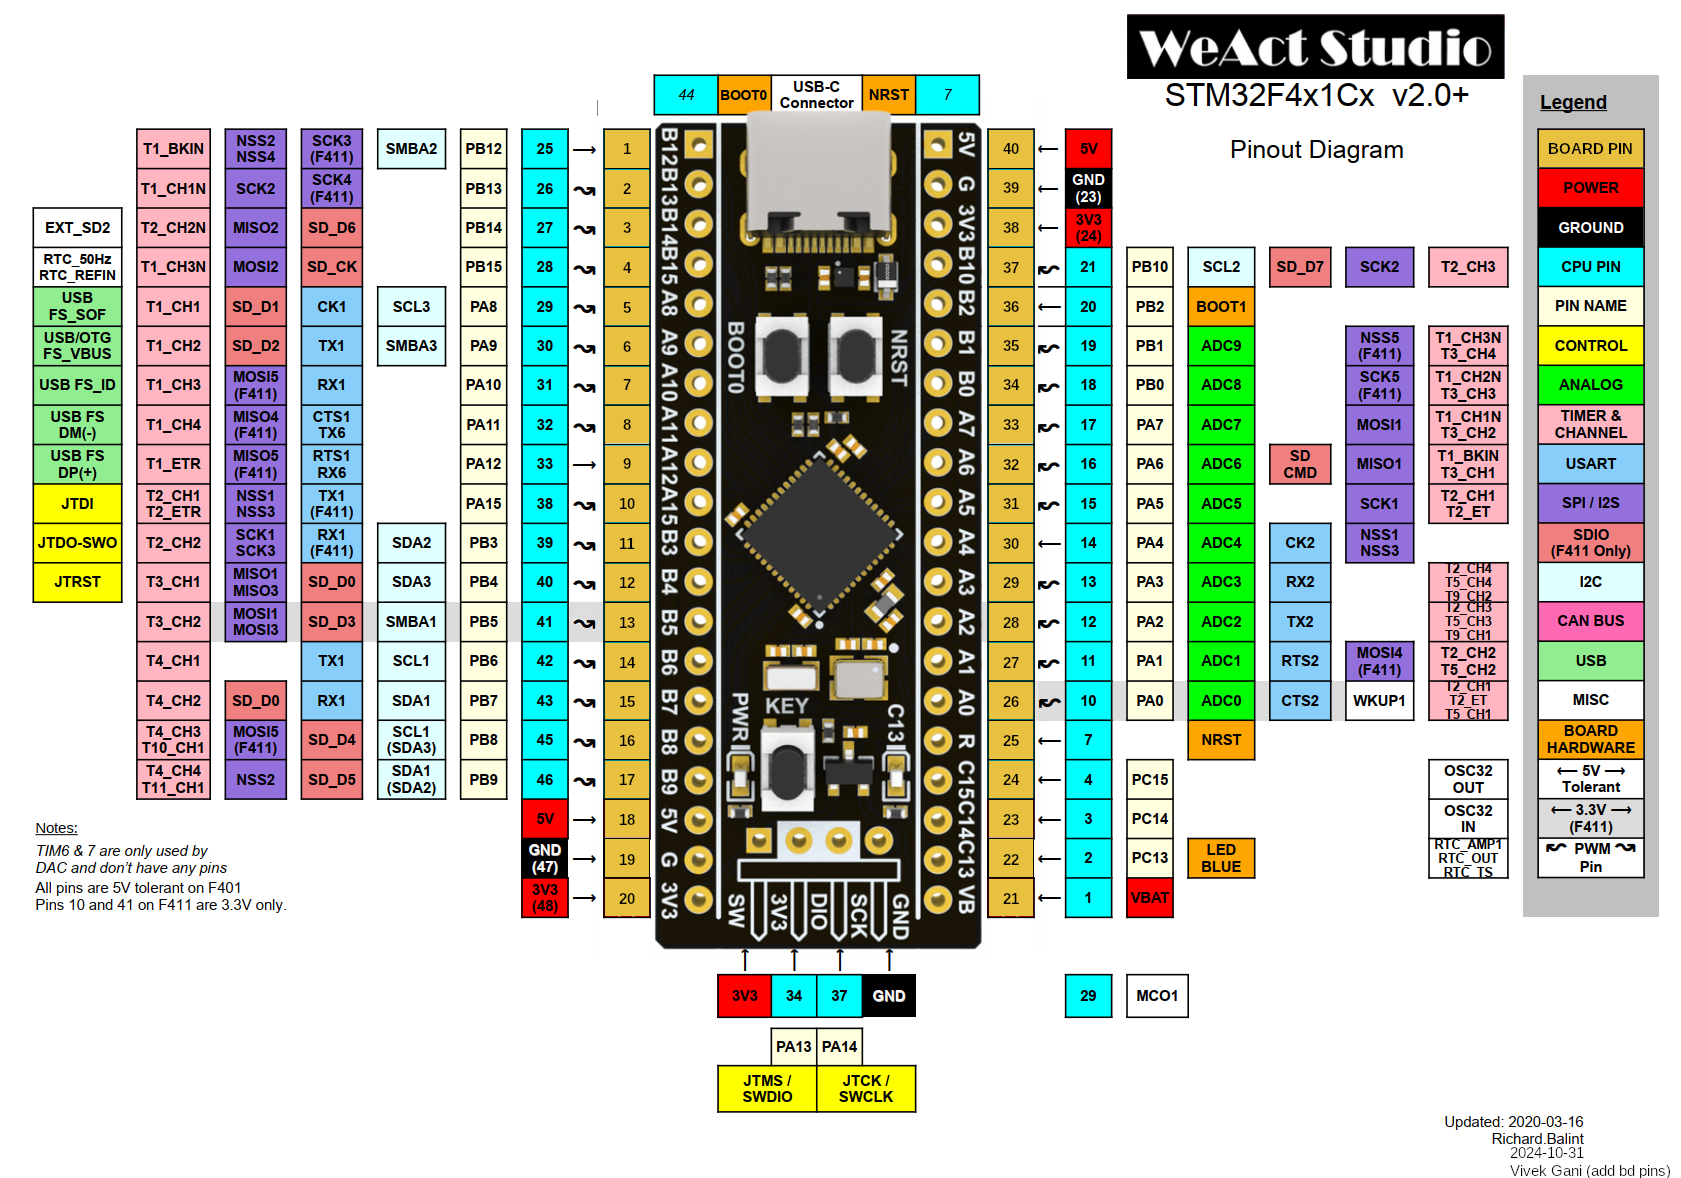
\includegraphics[width=0.8\textwidth]{images/hardware/STM32F4x1_PinoutDiagram_RichardBalint.png}
  \par\vspace{0.2cm}
  \footnotesize Fonte: WeActStudio, acesso em 22 abr. 2026.\footnote{Disponível em: \url{https://github.com/WeActStudio/WeActStudio.MiniSTM32F4x1}.}
\end{figure}

Com base na pinagem apresentada na Figura~\ref{fig:weact_github}, foram definidos os sinais utilizados pelo controlador de voo para comunicação com sensores, acionamento dos motores e troca de mensagens com o computador de missão. O Quadro~\ref{qua:pinos_stm32} resume os pinos reservados no protótipo e sua função na arquitetura embarcada.

\begin{quadro}[H]
  \centering
  \caption{Pinos da placa STM32F4x1 utilizados no protótipo.}
  \label{qua:pinos_stm32}
  \small
  \renewcommand{\arraystretch}{1.3}
  \begin{tabular}{|>{\centering\arraybackslash}p{2.4cm}|>{\raggedright\arraybackslash}p{10.5cm}|}
  \hline
  \textbf{Pinos usados} & \textbf{Função no protótipo} \\
  \hline
  PB10, PB3 & I$^2$C2 para IMU: SCL em PB10 e SDA em PB3. \\
  \hline
  PB4, PB5 & Interrupção e reset associados ao módulo BNO08X. \\
  \hline
  PB6--PB9 & Canais do TIM4 reservados para os quatro comandos DShot dos motores. \\
  \hline
  PA9, PA10 & USART1 para enlace UART com Raspberry Pi: TX em PA9 e RX em PA10. \\
  \hline
  PA2, PA3 & USART2 para o sensor MTF-01: TX em PA2 e RX em PA3. \\
  \hline
  PA4--PA7 & SPI1 para a memória \textit{flash} externa W25Q64: CS em PA4, SCK em PA5, MISO em PA6 e MOSI em PA7. \\
  \hline
  GND, 3V3, 5V & Referência comum e alimentação conforme os módulos conectados. \\
  \hline
  \end{tabular}
  \par\vspace{0.2cm}
  \footnotesize Fonte: elaborado pelos autores (2026).
\end{quadro}

% ----------------------------------------------------------------
\subsection{Sensores inerciais e de posição}\label{subsec:sensores}
% ----------------------------------------------------------------

A estimativa de estado do quadricóptero depende de dois sensores complementares:

\subsubsection{Unidade de Medição Inercial da família BNO08X}\label{subsubsec:bno08x}

O projeto adotou um módulo comercial BNO085, da família BNO08X. Essa família integra sensores inerciais e um hub de sensores capaz de disponibilizar \textit{reports} de aceleração, velocidade angular e vetores de rotação por meio da interface SH-2/SHTP \cite{bno08xdatasheet,sh2library}. A placa adquirida permite I$^2$C, e o projeto STM32 reserva I$^2$C2 a 400~kHz para essa interface.
Os vetores de rotação fornecidos pelo hub não dispensam a definição do estimador e dos sinais consumidos pelo controlador. O \textit{report} selecionado, taxa solicitada, taxa recebida, perda, \textit{jitter}, latência e comportamento sob vibração são medidos no conjunto real. Dessa maneira, limites de taxa publicados para uma saída específica não caracterizam garantia de que a malha completa opere nessa mesma frequência.

\subsubsection{Sensor de Fluxo Óptico e LiDAR MTF-01}\label{subsubsec:mtf01}

O MTF-01 é um módulo integrado que combina um sensor de fluxo óptico (PMW3901) e um LiDAR ToF (\textit{Time of Flight}) \cite{micoair2024}. O fluxo óptico mede movimento aparente da imagem; sua conversão em velocidade do veículo depende da distância ao solo, da orientação e da compensação da rotação. O LiDAR mede distância ao alvo no eixo de observação do sensor, que não coincide necessariamente com a altura vertical quando a aeronave está inclinada. O fabricante informa alcance de até 8~m sob condições especificadas, exatidão de 4~cm abaixo de 2~m a 90\% de refletância e 2\% acima de 2~m na mesma condição, além de alimentação de 5~V e interface UART a 115200~bit/s com protocolos Micolink, MAVLink e MSP \cite{micoairmtf01}. Assim, o MTF-01 fornece medições utilizadas na estimação e no controle de posição e altura, sem fornecer posição absoluta por si só.

\begin{figure}[H]
    \centering
    \caption{Pinagem do MTF-01.}
    \label{fig:mtf01}
    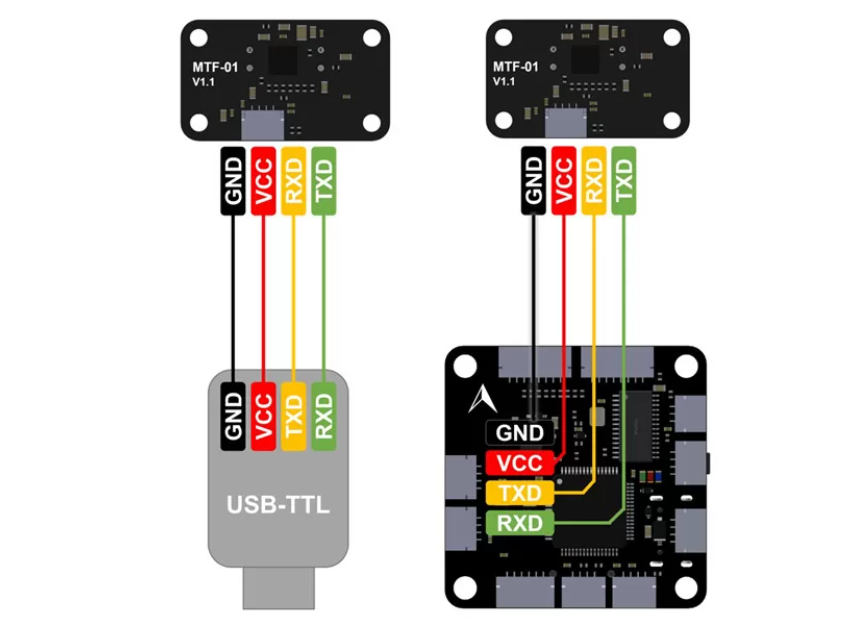
\includegraphics[width=0.5\textwidth]{images/hardware/MTF01Scheme.png}
    \fonte{MicoAir, acesso em 09 set. 2026.\footnote{Disponível em: \url{https://micoair.com/optical_range_sensor_mtf-01/}.}}
\end{figure}

O controlador atua sobre o estado estimado $\hat{\mathbf{x}}$, não sobre o estado verdadeiro diretamente. A arquitetura do protótipo deve registrar quais \textit{reports} do BNO08X são usados para atitude e velocidades angulares, como os eixos dos sensores são transformados para o referencial do corpo, como fluxo óptico e distância são convertidos em velocidade e posição relativa, como sinais com taxas diferentes são sincronizados, como a origem local é inicializada e como a deriva é tratada. Caso seja introduzido um estimador adicional no STM32, ele deve ser documentado como componente próprio, com parâmetros, taxas e método de validação.

% Protocolo MAVLink e comunicação confiável entre Raspberry Pi e STM32
% ============================================================================
% REFERENCIAL TEÓRICO — protocolo MAVLink e comunicação confiável entre o
% computador de missão e o controlador de voo.
% Chamado em partes/textuais/referencial_teorico.tex, na seção de sistemas
% embarcados e comunicação.
% ============================================================================

% ----------------------------------------------------------------
\subsection{Protocolo MAVLink}\label{subsec:mavlink}
% ----------------------------------------------------------------

O MAVLink (\textit{Micro Air Vehicle Link}) é um protocolo de mensagens binárias leve, projetado para sistemas com recursos limitados e enlaces de comunicação com largura de banda restrita \cite{koubaa2019, mavlinkguide}. É o protocolo utilizado pelos pilotos automáticos de código aberto PX4 e ArduPilot e por estações de solo como o QGroundControl, o que o tornou um padrão de fato na comunicação com VANTs \cite{koubaa2019}. Ele suporta fluxos periódicos de telemetria e microsserviços como missões, parâmetros e comandos; confirmações, retransmissões e semântica de conclusão dependem do microsserviço e da implementação adotada \cite{mavlinkguide}.

As mensagens são definidas em arquivos XML, que descrevem, para cada mensagem, seu identificador numérico, seus campos, os tipos e as unidades. O arquivo \texttt{common.xml} provê a maioria das mensagens utilizadas por pilotos automáticos e estações de controle, e um projeto pode criar um \textbf{dialeto} próprio, isto é, um XML que inclui o \texttt{common.xml} e acrescenta mensagens e enumerações específicas \cite{mavlinkguide}. A partir do XML, o gerador oficial (\texttt{mavgen}) produz o código de empacotamento e desempacotamento para diferentes linguagens; para sistemas embarcados como o STM32F411, a implementação de referência é uma biblioteca C \textit{header-only}, otimizada para o uso eficiente de RAM e \textit{Flash}, e, para Python, a biblioteca \texttt{pymavlink} \cite{koubaa2019, mavlinkguide}. Como os dois lados do enlace são gerados da mesma definição, a estrutura das mensagens é necessariamente a mesma em ambos.

No MAVLink 2, cada mensagem é transmitida em um pacote com a estrutura do Quadro~\ref{qua:mavlink_pacote}. O byte inicial permite ao receptor ressincronizar-se após a perda ou corrupção de bytes, procurando o próximo início de pacote; o número de sequência permite detectar pacotes perdidos; e os identificadores de sistema e componente indicam o remetente. Zeros no fim do \textit{payload} são omitidos na transmissão e restaurados na recepção, o que reduz o tamanho das mensagens \cite{mavlinkguide}.

\begin{quadro}[H]
    \centering
    \caption{Estrutura do pacote MAVLink 2.}
    \label{qua:mavlink_pacote}
    \small
    \renewcommand{\arraystretch}{1.3}
    \begin{tabular}{|>{\raggedright\arraybackslash}p{3.4cm}|>{\centering\arraybackslash}p{1.6cm}|>{\raggedright\arraybackslash}p{8.4cm}|}
        \hline
        \textbf{Campo} & \textbf{Bytes} & \textbf{Função} \\
        \hline
        Início (\texttt{0xFD}) & 1 & Marca o começo do pacote e permite a ressincronização. \\
        \hline
        Comprimento & 1 & Tamanho do \textit{payload}, de 0 a 255 \textit{bytes}. \\
        \hline
        \textit{Flags} & 2 & Indicações de compatibilidade, como o uso de assinatura. \\
        \hline
        Sequência & 1 & Contador de pacotes do remetente; saltos indicam perdas. \\
        \hline
        \textit{System ID} & 1 & Veículo ou sistema que enviou a mensagem. \\
        \hline
        \textit{Component ID} & 1 & Componente do sistema que enviou a mensagem. \\
        \hline
        \textit{Message ID} & 3 & Identificador da mensagem (até 16\,777\,215). \\
        \hline
        \textit{Payload} & 0 a 255 & Campos da mensagem em binário. \\
        \hline
        \textit{Checksum} & 2 & CRC-16/MCRF4XX do pacote, incluindo o \texttt{CRC\_EXTRA}. \\
        \hline
        Assinatura (opcional) & 13 & Autenticação da origem. \\
        \hline
    \end{tabular}
    \par\vspace{0.2cm}
    \footnotesize Fonte: elaborado pelos autores (2026), com base em \citeonline{mavlinkguide}.
\end{quadro}

No padrão MAVLink v1, o protocolo acrescenta 8~\textit{bytes} ao \textit{payload}. No MAVLink v2 sem assinatura, são acrescentados 12~\textit{bytes}; quando a assinatura opcional é usada, acrescentam-se mais 13~\textit{bytes}, totalizando 25~\textit{bytes} além do \textit{payload} \cite{mavlinkguide,mavlinksigning}. A integridade contra corrupção acidental é verificada por um \textit{checksum} CRC-16/MCRF4XX. O \texttt{CRC\_EXTRA}, um valor calculado a partir da definição da mensagem no XML, participa do cálculo desse \textit{checksum}: se emissor e receptor usarem definições diferentes para a mesma mensagem, o \textit{checksum} não confere e a mensagem é descartada, em vez de ser interpretada de forma errada. Ele não é um segundo \textit{checksum} transmitido separadamente \cite{mavlinkguide}.

Entre os microsserviços padronizados, destacam-se o \textit{HEARTBEAT}, mensagem periódica pela qual cada componente anuncia sua presença, seu tipo e seu estado, e cuja ausência indica a perda do enlace; o protocolo de comandos (\texttt{COMMAND\_LONG} e \texttt{COMMAND\_ACK}), em que cada comando recebe uma resposta com o resultado; e o protocolo de parâmetros (\texttt{PARAM\_*}), que permite ler e alterar valores de configuração do veículo durante a operação \cite{mavlinkguide}.

% ----------------------------------------------------------------
\subsection{Comunicação confiável entre o computador de missão e o controlador de voo}\label{subsec:comunicacao_confiavel}
% ----------------------------------------------------------------

Um enlace serial pode perder, corromper ou atrasar mensagens. O \textit{checksum} descarta mensagens corrompidas, mas não garante que uma mensagem chegue. Para que um comando seja executado com segurança, o protocolo de aplicação precisa de confirmações e de retransmissão: o emissor reenvia o pedido quando não recebe resposta dentro de um prazo. A retransmissão, porém, cria um problema: se o pedido foi executado e apenas a resposta se perdeu, o reenvio pode fazer o receptor executá-lo duas vezes \cite{tanenbaum2007}.

Para comandos que movem um veículo, a execução duplicada é inaceitável: um deslocamento de 1~m executado duas vezes leva o veículo a 2~m. A solução usual é tornar o pedido \textbf{idempotente}: cada pedido recebe um identificador único, o receptor guarda os pedidos já tratados e, ao receber um pedido repetido, apenas reenvia a resposta já dada, sem executá-lo de novo. Essa garantia é conhecida como semântica de \textbf{no máximo uma vez} (\textit{at-most-once}) \cite{tanenbaum2007}.

Também é necessário que o controlador de voo detecte a falha do computador de missão. Mensagens periódicas, como o \textit{HEARTBEAT}, funcionam como um \textit{watchdog} do enlace: se deixam de chegar por um tempo definido, o controlador assume que a comunicação foi perdida e executa uma ação segura, como manter a posição ou pousar \cite{mavlinkguide}. O mesmo princípio pode ser aplicado a uma autorização explícita do operador, renovada periodicamente, de forma análoga ao dispositivo de homem morto (\textit{dead man's switch}): o veículo só executa novos movimentos enquanto essa autorização continua a ser recebida.


% ----------------------------------------------------------------
\subsection{Protocolo DShot}\label{subsec:dshot}
% ----------------------------------------------------------------

O DShot (\textit{Digital Shot}) é um protocolo digital de comunicação entre o controlador de voo e os Controladores Eletrônicos de Velocidade (ESCs --- do inglês \textit{Electronic Speed Controllers}). Diferentemente dos protocolos analógicos tradicionais baseados em PWM (\textit{Pulse Width Modulation}), a trama possui 16~\textit{bits}: 11~\textit{bits} de valor, 1~\textit{bit} de solicitação de telemetria e 4~\textit{bits} de CRC. Os valores 0 e 1--47 são reservados; os comandos de \textit{throttle} ocupam a faixa 48--2047, totalizando 2000 níveis \cite{betaflightdshot}.

As principais vantagens do DShot sobre protocolos analógicos são \cite{idrissi2022}:

\begin{alineastcc}
    \item \textbf{verificação de integridade}: a codificação digital e o CRC ajudam a detectar erros de transmissão, embora o sinal continue sujeito a ruído, problemas de temporização e falhas elétricas;
    \item \textbf{resolução}: 2000 níveis de \textit{throttle} úteis, além dos valores reservados do protocolo;
    \item \textbf{ausência de calibração dos extremos de \textit{throttle}}: não é necessário definir pulsos mínimo e máximo como em protocolos PWM, embora a configuração do ESC e a caracterização de empuxo permaneçam necessárias;
    \item \textbf{temporização definida}: variantes como DShot600 usam taxa de linha de 600~kbit/s; a frequência prática de atualização depende da versão, da telemetria e da implementação \cite{betaflightdshot}.
\end{alineastcc}

No STM32F411, a implementação utiliza temporizador e DMA (\textit{Direct Memory Access}) para reduzir a intervenção do processador na transmissão. A compatibilidade entre o período da malha e a geração do sinal depende da medição elétrica do DShot e da integração com o ESC.
